% vim: set spelllang=fr foldmethod=marker:
\chapter{Structure du réseau et hypothèses de travail}\label{chap:st}

% préfixe: st
\renewcommand\chapterpath{Main/Structure}
\renewcommand\chapterfig{Main/Structure/Figures}

% vim: set spelllang=fr foldmethod=marker:
\section{Réseaux de capteurs sans fil}
\label{st:sec:contexte}

    \subsection{De quoi s'agit-il?}
%{{{1
%{{{2
\begin{figure}[!b]
    \centering
    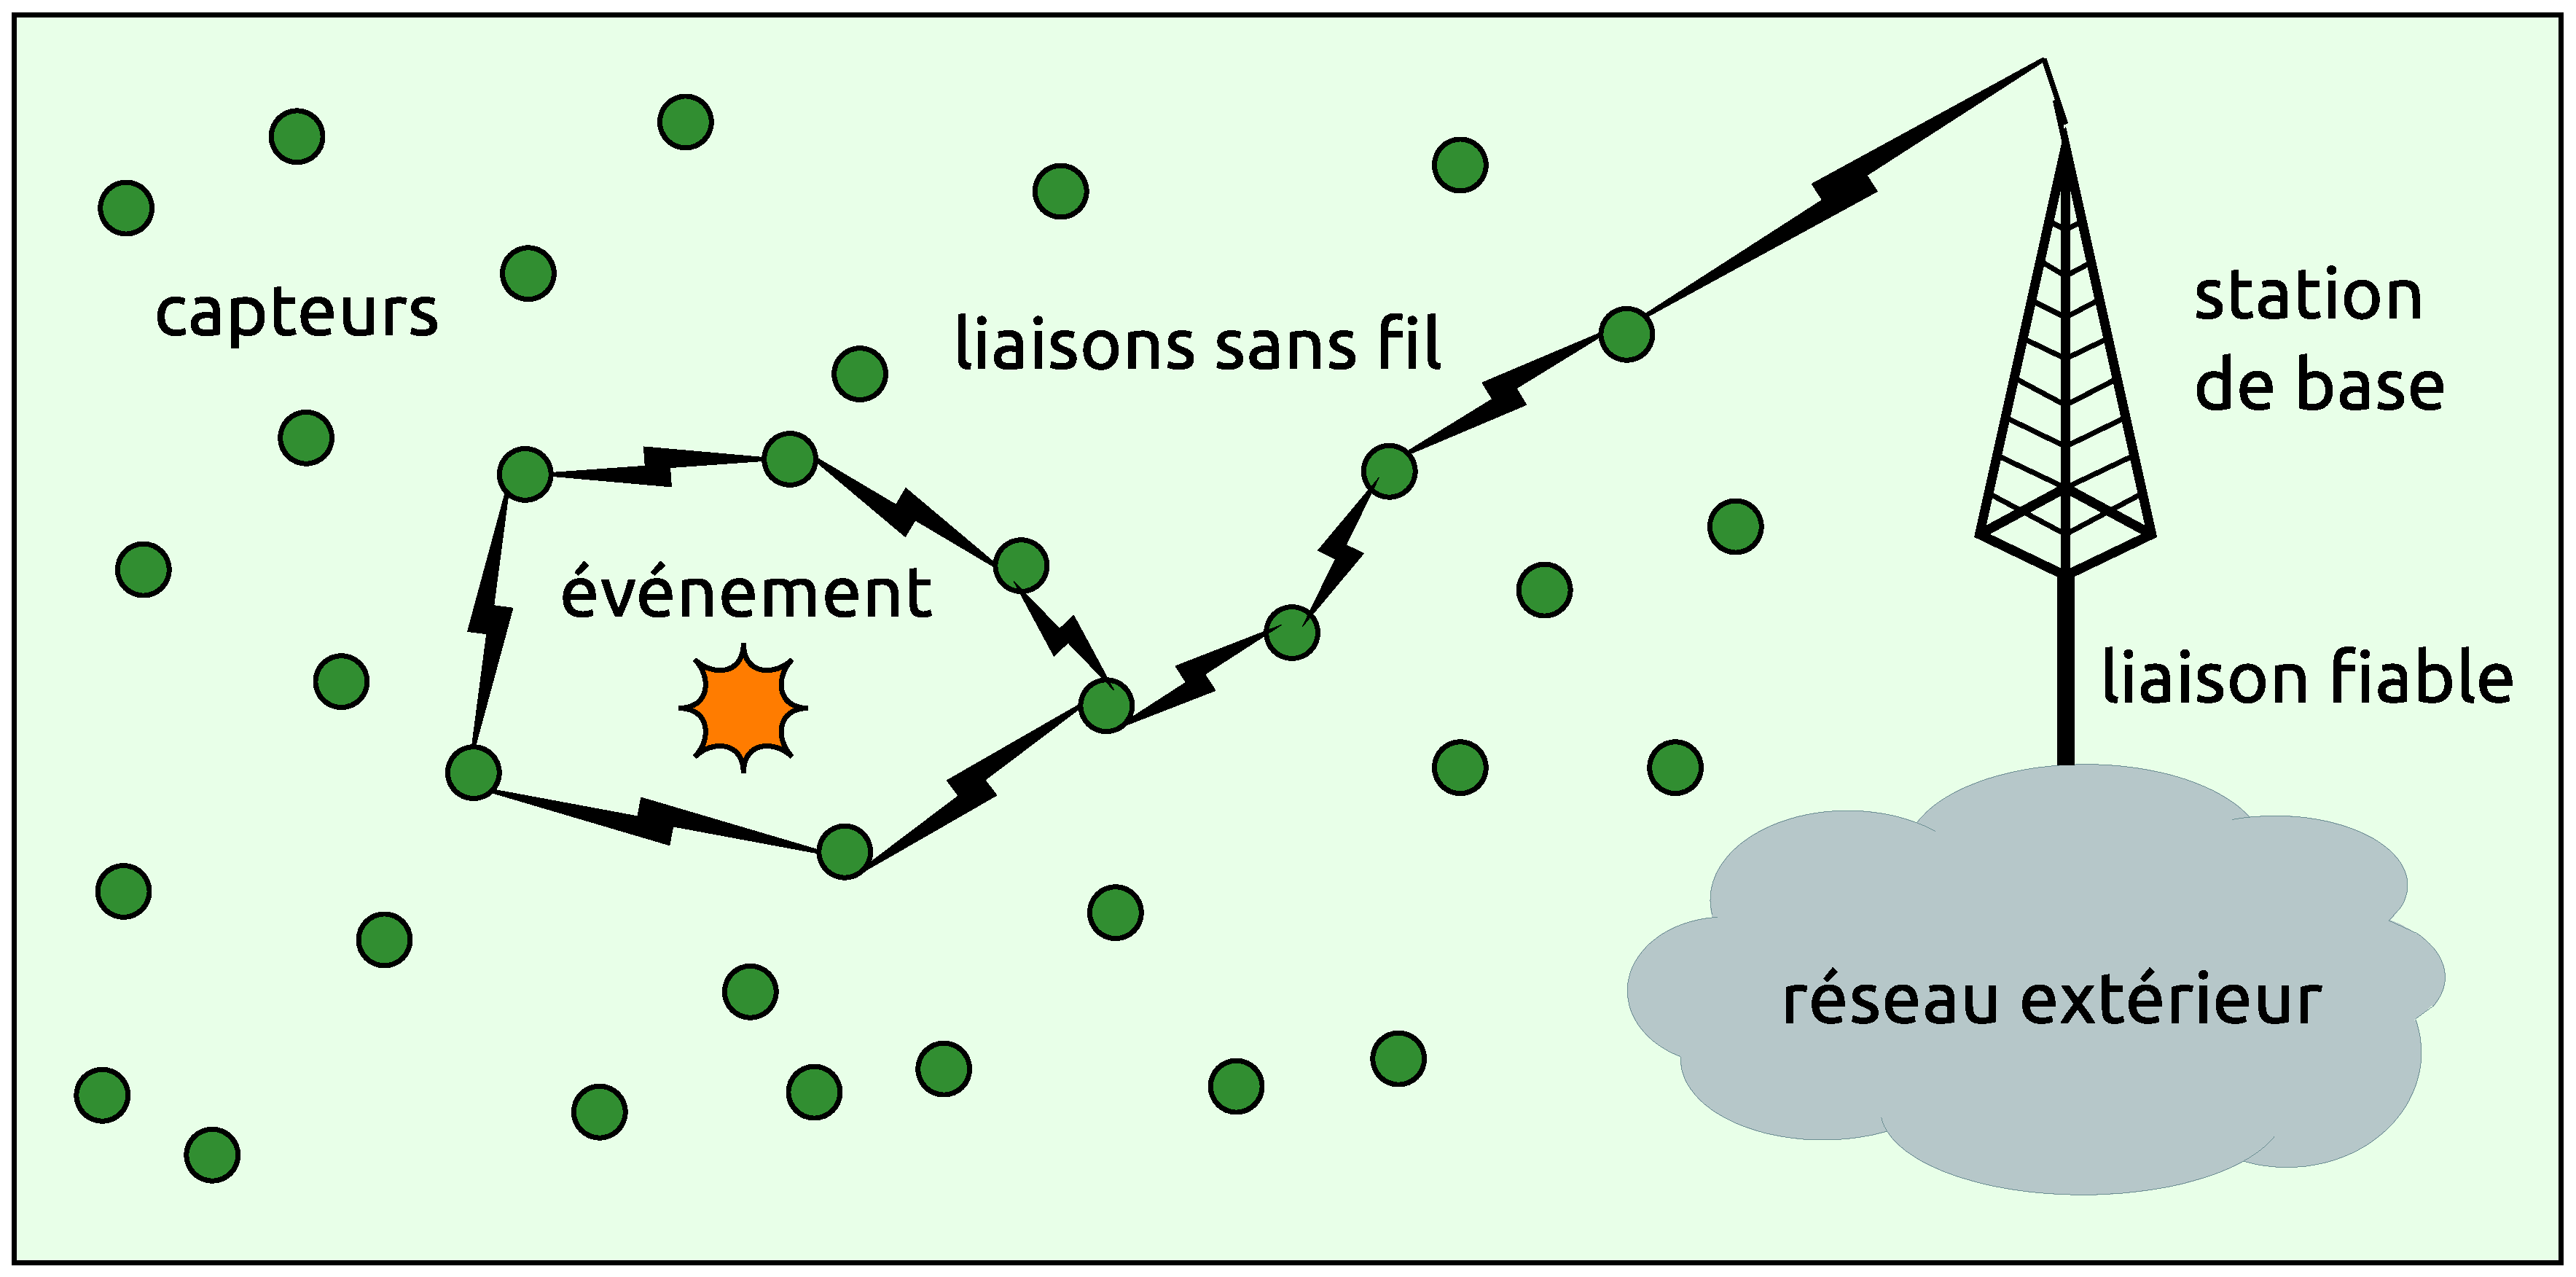
\includegraphics[width=.8\textwidth]{\chapterpath/Figures/WSN_archi.eps}
    \caption{Schéma simple d'un \rcsf}\label{st:fig:wsnintro}
\end{figure}
Les \rcsfs, ou \textit{\WSN} (pour \wsns en anglais), sont des réseaux constitués de petits appareils, les capteurs, ainsi que d'une \sdb.
\nomenclature{WSN}{\wsns}
Les capteurs échangent par communications hertziennes, en utilisant des protocoles tels ceux définis dans la pile \ieeee.
Le routage des paquets dans le réseau peut faire appel à l'un des nombreux protocoles développés à cet effet (par exemple: \aodv, \olsr), qu'il repose sur un algorithme centralisé (dirigé par une seule entité) ou distribué (exécuté par chaque entité du réseau).
Les capteurs collectent des informations sur leur environnement et les font remonter à la \sdb.
Cette \sdb, ou \BS (pour \bs), ou encore parfois \textit{puits} (\textit{sink} en anglais), est chargée de récolter et traiter les données provenant des capteurs.
Une fois les capteurs déployés, l'administrateur n'interagit plus avec le réseau que par le biais de la \sdb.
Un schéma basique de \rcsf est présenté en \figref{st:fig:wsnintro}
\nomenclature{BS}{\bs}

Il est rare que tous les capteurs d'un \WSN soit directement connectés les uns aux autres.
À la topologie d'un réseau donné est donc très souvent associé le graphe de connectivité du réseau.
Pour cette raison, il est souvent fait référence aux capteurs sous le terme de \textit{nœuds} (ou de \textit{nodes} en anglais).

\begin{figure}[H]
    \centering
    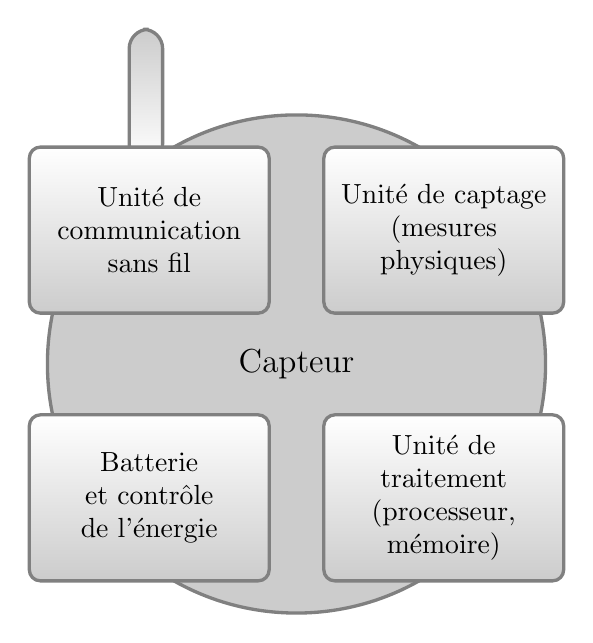
\begin{tikzpicture}[%
        scale=.85,
        sensor/.style={%
            circle,%
            minimum size=18em,%
            very thick,%
            draw=black!50, %
            fill=black!20%
        },%
        module/.style={%
            rounded corners,%
            text width=8em,%
            minimum height=6em,%
            align=center,%
            very thick,%
            draw=black!50, %
            top color=white,%
            bottom color=black!20%
        }%
    ]
    \node (sensor) at (   0, 0) [sensor]{\large Capteur};
    \draw [rounded corners=7pt,top color=black!20,draw=black!50,very thick] (-2,3)--(-2,5)--(-2.5,5)--(-2.5,3)--cycle ;
    \node (mesure) at ( 2.2, 2) [module]{Unit\'e de captage\\(mesures physiques)};
    \node (mesure) at (-2.2, 2) [module]{Unit\'e de\\communication sans fil};
    \node (mesure) at ( 2.2,-2) [module]{Unit\'e de traitement\\(processeur, m\'emoire)};
    \node (mesure) at (-2.2,-2) [module]{Batterie\\et contr\^ole de l'\'energie};
    \end{tikzpicture}
    \caption{Schéma représentant les principaux modules d'un capteur standard}\label{st:fig:sensor}
\end{figure}
Un capteur seul peut être vu comme l'assemblage de quatre modules principaux, représentés en \figref{st:fig:sensor}.
Il s'agit:
\begin{itemize}
    \item d'une unité de captage, chargée de réaliser des mesures physiques (analogiques) sur l'environnement, puis de les convertir en un signal numérique;
    \item d'un module de traitement, composé principalement d'un processeur et de mémoire (mémoire vive et mémoire non volatile), qui assure le fonctionnement du système d'exploitation, gère les interactions entre les différents modules, et surtout traite les données récoltées;
    \item d'une unité de transmission/réception utilisée pour les communications hertziennes;
    \item d'une batterie, accompagnée d'une unité de contrôle de l'énergie elle-même chargée d'alimenter de façon efficace les autres modules du capteur.
\end{itemize}
%2}}}
%1}}}

    \subsection{Applications}
%{{{1
Le champ d'application des \WSN est très vaste, et n'a de cesse de s'élargir au fil du temps et des avancées technologiques.
Toutes ne font pas l'objet de publications scientifiques, mais certaines sont régulièrement évoquées en tant qu'exemples, ou bien font l'actualité dans le domaine des nouvelles technologies voire le domaine commercial.

        \paragraph{Applications environnementales}
%{{{2
La gestion de l'environnement par l'Homme a de plus en plus recours à des mesures distribuées reposant sur l'usage de capteurs.
Les prévisions météorologiques (reposant sur des mesures d'hygrométrie, de pression de l'air, \etc) ont été l'un des premiers champs d'application des capteurs.
Les mesures de qualité de l'air et de taux de pollution, en ville comme en campagne, se généralisent peu à peu.
Les réseaux de capteurs permettent même de pousser la mesure de ce taux vers de nouveaux milieux, comme les glaciers~\cite{MPROH05} ou bien les océans.

L'agriculture est également susceptible d'avoir recours aux capteurs: des essais sont menés sur la réalisation de mesures faites par des microcapteurs semés en même temps que les cultures, permettant de surveiller au mieux les conditions de développement de ces dernières.
Placés judicieusement dans l'habitat naturel de certaines espèces, les capteurs peuvent être utilisés pour suivre et analyser le comportement de la faune d'un milieu~\cite{KDA14}.

En forêt, les \rcs peuvent permettre de détecter les départs de feu et de lutter plus efficacement contre les incendies.
Et en zones à risques, ils peuvent être utilisés pour mesurer l'activité sismique ou volcanique du sol, et permettre une meilleure anticipation des phénomènes naturels.
L'industrie a également recours à ces réseaux pour détecter d'éventuelles fuites de produits toxiques (pétrole, gaz, éléments radioactifs).

Il est à noter que certaines de ces applications touchent à des domaines critiques (en termes de sécurité des installations, voire de vies humaines): il est indispensable d'assurer le bon fonctionnement du réseau déployé dans un tel contexte.
%2}}}

        \paragraph{Surveillance et détection}
%{{{2
Les \rcsfs sont aussi employés pour des mesures de sureté ou de sécurité, par exemple pour surveiller l'intégrité structurelle de certaines architectures (ferroviaires, aérospatiales, maritimes, ou plus simplement dans le bâtiment: gros œuvre, ouvrages d'art) et peuvent permettre une prévention efficace des pannes matérielles~\cite{SCOA13}.
Mis à part la détection de pannes, les capteurs peuvent être utilisés dans des systèmes de surveillance de sites sensibles afin de prévenir les intrusions humaines, ou bien pour détecter des incidents ou encore établir le suivi de certaines entités; la gestion du trafic routier, ou même seulement des autobus, en sont des exemples.
Le CEREMA (Centre d'études et d'expertise sur les risques, l'environnement, la mobilité et l'aménagement) a mis en ligne un site Internet particulièrement riche en exemples d'application des capteurs, et détaillant notamment les différentes technologies utilisées pour réaliser les mesures~\cite{sti}.
Pour exemple la seule détection de véhicules sur les voies de circulation peut reposer sur:
\begin{itemize}
    \item la détection d'une modification du champ magnétique environnant;
    \item la pression exercée par le véhicule sur la voie;
    \item la variation de la pression dans un tube pneumatique;
    \item les déformations de la structure d'un pont sous le poids des véhicules;
    \item les variations d'intensité lumineuse ou sonore;
    \item le renvoi d'ondes radar, ou lumineuses (laser), ou infrarouges, ou ultrasons;
    \item l'analyse d'image vidéo visibles ou infrarouges, par reconnaissance de forme, ou bien par détection du mouvement des groupes de pixels…
\end{itemize}
\nomenclature{laser}{\textit{Light Amplification by Stimulated Emission of Radiation}}
\nomenclature{radar}{\textit{RAdio Detection And Ranging}}

Également en milieu urbain, les applications de vidéosurveillance font de plus en plus appel à des capteurs en réseau~\cite{SZFDXC14}.
%2}}}

        \paragraph{Domaine militaire}
%{{{2
La surveillance et la détection sont aussi très utilisés dans le domaine militaire.
Qu'il s'agisse de mener des opérations de renseignement ou bien de suivre l'évolution d'un combat sur le champ de bataille, pour analyser les cibles, relier entre eux fantassins et véhicules de tous types, pour détecter les agents radioactifs, chimiques ou biologiques répandus par un ennemi, toutes les informations sont bonnes à prendre~\cite{ASSC02}.
Un maximum d'entre elles doivent être remontées au centre de commandement, afin de permettre une supervision optimale des forces en mouvement.

Plus encore que les exemples précédents, l'usage des capteurs en contexte militaire implique de fortes contraintes en termes de \secu du réseau déployé.
%2}}}

        \paragraph{Médecine}
%{{{2
Certains usages des capteurs tiennent du domaine médical~\cite{SZFDXC14}.
Il peut s'agir par exemple de faire communiquer un ou plusieurs implants avec un contrôleur externe.
Il peut également être question d'employer des microcapteurs pour analyser avec précisions des variables corporelles (taux de glycémie, surveillance des organes vitaux) ou bien, sur une plus courte durée, pour traiter avec précision une pathologie locale (des cellules cancéreuses par exemple).
%2}}}

        \paragraph{Grand public}
%{{{2
Le public a lui aussi de plus en plus accès à des applications reposant sur les capteurs.
En domotique par exemple, la température des différentes pièces d'un lieu d'habitation peut être rendue accessible à tout instant, tandis que des fonctions comme l'activation de volets électriques, l'ouverture de portes, l'activation de sources lumineuses ou de dispositifs de chauffage peuvent être effectuées à distance par l'habitant (par exemple par le biais d'une application logicielle sur téléphone portable) ou bien de façon automatique en fonction des besoins identifiés à partir des données récoltées~\cite{ASSC02}.

Un autre domaine d'application en voie de développement est ce que l'on appelle l'\textit{\idx{Internet des objets}} (\textit{the Internet of things} en anglais), et qui consiste en quelque sorte à étendre \idx{Internet} au monde réel, par le biais d'une interconnexion réseau entre les objets de la vie courante: de plus en plus d'objets du quotidien tendent à devenir « connectés ».
Ils se voient alors équipés de capteurs, d'un module de communication sans fil, et offrent de nouvelles possibilités en termes d'usages.
En voici quelques exemples:
\begin{itemize}
    \item les montres (interfacées avec les téléphones « intelligents » pour afficher des notifications diverses);
    \item les ampoules d'éclairage (gestion de la luminosité, de la couleur de l'éclairage, parfois dynamiques);
    \item les ceintures (accessoires vestimentaires: réajustement automatique du réglage, collecte de données sur le tour de taille pour le contrôle du poids);
    \item les réfrigérateurs (gestion des réserves alimentaires, création de listes d'achat);
    \item les véhicules autonomes, tels que les voitures sans conducteurs ou les drones (pilotage de l'engin, relevé de mesures tactiques pour les drones militaires).
\end{itemize}
Des puces RFID (de l'anglais \textit{Radio Frequency Identification}, « identification sur fréquences radio ») se retrouvent par ailleurs de plus en plus utilisées, entre autres raisons pour faciliter de telles interactions dans le monde « connecté »~\cite{TW10}.
Au fur et à mesure que ces objets intègrent la vie quotidienne des utilisateurs, ils auront probablement tendance à communiquer de plus en plus entre eux, entre objets, en ne centralisant les données que sur une seule interface présentée à l'utilisateur final.
\nomenclature{RFID}{\textit{Radio Frequency IDentification}}
%2}}}

        \paragraph{}
Les applications présentées ici ne représentent bien sûr que quelques exemples parmi les nombreux usages existants des capteurs~\cite{ASSC02}, dont la quantité ne cesse par ailleurs de croitre au fil du temps.
%1}}}

    \subsection{Contraintes en ressources}
%{{{1
De par leur petite taille, et à cause de leurs déploiement dans des zones souvent difficiles d'accès, les capteurs n'embarquent qu'une quantité limitée de matériel, qui ne peut pas toujours être remplacé.
Les capteurs se retrouvent donc avec des capacités limitées~\cite{BMS13}, notamment en ce qui concerne:
\begin{itemize}
    \item les \textbf{capacités de calcul}: les processeurs embarqués sont relativement peu puissants, principalement pour des raisons de cout.
        Les algorithmes exécutés par les capteurs doivent donc être de complexité relativement basse;
    \item les \textbf{capacités de mémoire}: les capteurs disposent de mémoire vive (RAM, \textit{Random Access Memory}, « mémoire à accès non séquentiel » en anglais) et d'un peu d'espace de stockage, mais ils ne sont pas du tout conçus pour sauvegarder de grandes bases de données.\nomenclature{RAM}{\textit{Random Access Memory}}
        Les informations récoltées doivent être acheminées à la \sdb, et non stockées sur le long terme par les capteurs eux-mêmes;
    \item l'\textbf{énergie disponible}: les capteurs disposent d'une batterie qui leur fournit une quantité d'énergie finie, et (la plupart du temps) non rechargeable.
        Il est donc essentiel de conserver à l'esprit une gestion parcimonieuse de l'énergie pour tout programme implémenté sur les capteurs.
        Des calculs importants, ainsi que des émissions/réceptions d'ondes électromagnétiques nombreuses ou mal gérées, sont les principaux facteurs d'un épuisement prématuré de la batterie.
\end{itemize}

Il est à noter qu'au regard de ces contraintes qui affectent les capteurs, la \sdb est considérée comme disposant de capacités « illimitées ».
%1}}}

\pagebreak %%%%%%%%%%%%%%%%%%%%%%%%%%%%%%%%%%%%%%%%%%%%%%%%%%%%%%%%%%%%%%%%%%%%
    \subsection{Communications sans fil}
%{{{1
%{{{2
Comme l'indique leur nom, les \rcsfs n'utilisent aucun câble physique pour communiquer entre eux ou avec la \sdb: toutes les transmissions sont effectuées par voie hertzienne.
Chaque capteur est équipé d'un module radio utilisé alternativement pour émettre et pour recevoir.
La plupart du temps ces modules sont capables de changer de fréquence de communication, ainsi que de moduler la puissance d'émission utilisée pour les transmissions.

Les protocoles de communication déployés sur cette architecture sont multiples (on parle d'\textit{encapsulation} des données).
Il faut pouvoir communiquer de pair à pair entre nœuds voisins, tout comme il faut être capable de faire parvenir un message à un nœud éloigner en faisant retransmettre les paquets par des nœuds relais successifs, d'assurer certains services comme le maintien de session, ou de gérer des applications.
Comme dans la plupart des réseaux informatiques, l'empilement des protocoles reprend donc le modèle \tcpip~\cite{TW10} (schéma concret lui-même issu du modèle théorique \idx{OSI}, de l'anglais \textit{Open Systems Interconnection}), présenté en \figref{st:fig:tcpip}.
\nomenclature{OSI}{\textit{Open Systems Interconnection}}
\begin{figure}[H]
    \centering
    \begin{tabular}{c |c| l}
        \multicolumn{2}{c}{} & Exemples:\\
        \cline{2-2}
        5 & Application & HTTP, FTP, SSH\\
        \cline{2-2}
        4 & Transport   & TCP, UDP\\
        \cline{2-2}
        3 & Réseau      & IP\\
        \cline{2-2}
        2 & Liaison     & \ieeee (\csmaca)\\
        \cline{2-2}
        1 & Physique    & ondes électromagnétiques\\
        \cline{2-2}
     \end{tabular}
    \medskip
    \caption{Modèle TCP/IP}\label{st:fig:tcpip}
\end{figure}
\nomenclature{TCP}{\textit{Transmission Control Protocol}}
\nomenclature{IP}{\textit{Internet Protocol}}
\nomenclature{UDP}{\textit{User Datagram Protocol}}
\nomenclature{HTTP}{\textit{HyperText Transfer Protocol}}
\nomenclature{FTP}{\textit{File Transfer Protocol}}
\nomenclature{SSH}{\textit{Secure SHell}}

Certains standards normalisés définissent l'usage de protocoles spécifiques sur les trois premières couches.
Les principaux standards qui sont employés dans les \rcs sont les piles \ieeee (correspondant à la marque \wifi) et \ieeeff (sur laquelle sont basée la marque \zigbee et le standard \ietf \slowpan), et dans une moindre mesure la pile \ieeefo (correspondant à la marque \bluetooth).
\nomenclature{IETF}{\textit{Internet Engineering Task Force}}
\nomenclature{IEEE}{\textit{Institute of Electrical and Electronics Engineers}}
\nomenclature{6LoWPAN}{\textit{IPv6 over Low power Wireless Personal Area Networks}}
%2}}}

            \paragraph{La couche physique}
%{{{2
Cette couche concerne l'émission et la réception en soi des ondes électromagnétiques, et l'encodage utilisé pour leur faire porter des valeurs numériques (par opposition à un signal analogique)~\cite{TW10}
Les réseaux sans fil ont la particularité de ne pas pouvoir restreindre l'envoi d'un paquet vers son seul destinataire: un paquet émis par transmission électromagnétique est reçu par tout nœud voisin (\cad à distance suffisamment faible pour être couvert par la portée d'émission de l'émetteur) qui écoute le canal (donc les plages de fréquences concernées) au moment de la transmission.
Il est parfois possible de se servir d'une \idx{antenne directionnelle} pour réduire sensiblement les directions dans laquelle est réalisée la diffusion et pour augmenter le ratio de la puissance du signal émis sur l'énergie consommée par l'envoi; mais cet équipement couteux n'est que très rarement utilisé dans les réseaux de capteurs.

Une propriété fréquemment employée en revanche est la capacité à moduler la puissance du signal en fonction des besoins.
Plus le signal est fort, plus il portera loin (et permettra d'atteindre des nœuds distants).
Naturellement, l'émission consommera également plus d'énergie
%2}}}

            \paragraph{La couche de liaison de données}\label{st:ssec:mac}
%{{{2
La deuxième couche du modèle fournit les moyens fonctionnels et procéduraux pour le transfert des données entre deux entités du réseau~\cite{TW10}.
Elle permet aussi, le plus souvent, de détecter et éventuellement corriger certaines erreurs survenues sur la couche physique (en cas de perturbation ou dégradation du signal électromagnétique).
Elle se décompose en deux sous-couches: la couche de contrôle de la liaison logique (\llc, pour \textit{Logical Link Control} en anglais, « contrôle de la liaison logique ») et la couche du contrôle d'accès au support (\mac, pour \textit{Media Access Control}, « contrôle d'accès au support »).
\llc est la sous-couche haute, utilisée pour fiabiliser la sous-couche \mac, intervient peu dans les \rcs.
Le protocole de couche \mac définit la manière dont les différents agents du réseau accèdent au médium de transmission de façon à limiter les collisions, et à garantir un accès le plus souvent équivalent au médium pour tous les nœuds.
Les différents modes d'accès au médium existants sont résumés dans la \tabref{st:tab:mac}; certains consistent à créer des canaux de transmission distincts, tandis que d'autres déterminent l'accès à une même bande de fréquence en instaurant des règles.
\nomenclature{MAC}{\textit{Media Access Control}}
\nomenclature{LLC}{\textit{Logical Link Control}}

\begin{table}[!ht]
    \caption{Méthodes d'accès au médium de transmission}\label{st:tab:mac}
    \centering
    \medskip
    \begin{small}
        \begin{tabular}{m{.2\textwidth}|m{.2\textwidth}|m{.48\textwidth}}
            \toprule
            \textsc{Nom anglais} & \textsc{Traduction} & \textsc{Description}\\
            \midrule
            \multicolumn{3}{c}{Commutation de circuits et création de canaux}\\
            \midrule
            \textit{Frequency Division Multiple Access} (\fdma) & Accès multiple par répartition en fréquence & Plusieurs canaux basés sur des fréquences différentes\\
            \midrule
            \textit{Code division multiple access} (\cdma) & Accès multiple par répartition en code & Étalement du spectre de fréquence utilisé en conjonction avec techniques comme les sauts de fréquences ou la génération de bruit pseudo-aléatoires (avec la même séquence pseudo-aléatoire appliquée au signal côté émetteur comme côté destinataire)\\
            \midrule
            \textit{Time division multiple access} (\tdma) & Accès multiple à répartition dans le temps & Un seul canal dont l'accès est réparti par créneaux dans le temps\\
            \midrule
            \textit{Space division multiple access} (\sdma) & Accès multiple à répartition dans l'espace & Plusieurs canaux spatiaux obtenus à l'aide d'antennes directionnelles. À noter: les antennes directionnelles augmentent sensiblement le cout de production des capteurs.\\
            \midrule
            \multicolumn{3}{c}{Mode d'accès par paquet}\\
            \midrule
            \textit{Contention based random multiple access methods} & Accès par contention & Contention par le nœud du paquet à envoyer jusqu'à ce que le protocole le lui autorise. Dans cette catégorie se trouve notamment le protocole \csmaca (\textit{Carrier Sense Multiple Access with Collision Avoidance}, accès multiple par écoute du canal avec esquive de collision), très utilisé dans les réseaux sans fil (\ieeee entre autres).\\
            \midrule
            \textit{Resource reservation (scheduled) packet-mode protocols} & Réservation des ressources & Réservation par un nœud des ressources (par exemple: créneau temporel) nécessaires à la transmission)\\
            \midrule
            \multicolumn{3}{p{.95\textwidth}}{D'autres modes d'accès par paquet (\textit{token passing, polling}) existent mais ne sont pas utilisés dans les \rcs}\\
            \bottomrule
         \end{tabular}
     \end{small}
\end{table}
\nomenclature{FDMA}{\textit{Frequency Division Multiple Access}}
\nomenclature{CDMA}{\textit{Code Division Multiple Access}}
\nomenclature{SDMA}{\textit{Space Division Multiple Access}}
\nomenclature{TDMA}{\textit{Time  Division Multiple Access}}
\nomenclature{CSMA}{\textit{Carrier Sense Multiple Access}}
\nomenclature{CSMA/CA}{\textit{Carrier Sense Multiple Access with Collision Avoidance}}

De ces modes d'accès sont dérivés de très nombreux protocoles de couche \mac, dont plusieurs ont été conçus spécifiquement pour les \rcs~\cite{YB09}.
Par exemple, en dehors des standards \ieee, le protocole \smac~\cite{YHE02} fait alterner périodes « actives » et périodes de sommeil aux capteurs afin de préserver leur batterie.
Les capteurs sont associés dans des groupes (qui ne correspondent pas tout à fait à des clusters) dont tous les membres sont en éveil de manière simultanée, afin de pouvoir communiquer à l'aide d'une version modifiée de \csmaca tel que défini dans le standard \ieeee.
\nomenclature{S-MAC}{\textit{Sensor-MAC}}
%2}}}

            \paragraph{La couche réseau}
%{{{2
Cette couche, pour les capteurs sans fil, repose le plus souvent sur le protocole \ip (\textit{Internet Protocol} an anglais), que ce soit en version 4 ou 6 (la version 6 est notamment utilisée avec la pile \slowpan), pour l'adressage, et sur un protocole de routage qui détermine comment les paquets sont retransmis saut après saut dans le réseau~\cite{TW10}.

Les \rcsfs composent en quelque sorte une sous-famille des réseaux sans fil \adhoc (ou \wanet, de l'anglais \textit{wireless Ad hoc Network}), et une grande partie des protocoles et algorithmes utilisés proviennent du monde des \wanet.
Des exemples classiques de ces algorithmes de routage incluent \aodv (\textit{Ad hoc On-Demand Distance Vector Routing})~\cite{aodv} ou son évolution \dsr~\cite{dsr} (\textit{Dynamic Source Routing}), \olsr~\cite{olsr} (\textit{Optimized Link State Routing Protocol}) ou ses évolutions \dsdv (\textit{Destination-Sequenced Distance Vector routing}) et \batman (\textit{Better Approach To Mobile Adhoc Networking}), \etc.
Ces protocoles se répartissent le plus souvent en deux grandes classes: les protocoles « proactifs » reposant sur une table de \idx{routage} établie \apriori, en amont des requêtes (\aodv par exemple); et les protocoles de routage « à la demande » (dont \olsr), qui établissent les routes à la volée lorsqu'une requête de retransmission parvient au nœud relais.
\nomenclature{AODV}{\textit{Ad hoc On-demand Distance Vector routing}}
\nomenclature{DSR}{\textit{Dynamic Source Routing}}
\nomenclature{OLSR}{\textit{Optimized Link State Routing protocol}}
\nomenclature{DSDV}{\textit{Destination-Sequenced Distance Vector routing}}
\nomenclature{B.A.T.M.A.N.}{\textit{Better Approach To Mobile Adhoc Networking}}
\nomenclature{WANET}{\textit{Wireless Ad hoc NETwork}}
%2}}}

            \paragraph{La couche transport}
%{{{2
Cette couche gère les communications de bout en bout entre processus.
Les protocoles les plus fréquemment utilisés, \tcp (\textit{Transmission Control Protocol}) et \udp (\textit{User Datagram Protocol}) assurent l'ordonnancement des paquets et permettent d'éviter les pertes, les doublons et la corruption des paquets~\cite{TW10}.
Le protocole \tcp permet en plus à deux entités de communiquer en mode connecté en établissant une session (début, fin et validation des échanges).
En raison des données de contrôle que ces protocoles impliquent, ils ne sont pas systématiquement implémentés dans les \rcs (ils le sont parfois dans des versions allégées).
%2}}}

            \paragraph{La couche application}
%{{{2
La dernière couche gère les échanges applicatifs entre les différents agents du réseau, et encapsule les données utiles au format désiré pour leur traitement final~\cite{TW10}.
Il s'agit de la couche la plus haut niveau  du modèle.
Elle assure un service propre à l'application déployée, et les protocoles déployés à ce niveau dépendent donc totalement de l'objectif final du réseau, il n'y a donc pas de standard propre aux \rcs.
%2}}}
%1}}}

    \subsection{Terminologie employée}
%{{{1
            \paragraph{Capteurs et nœuds}
%{{{2
Un \rcsf est souvent représenté sous forme de graphe.
En conséquence, il est souvent fait références aux capteurs eux-mêmes sous le terme de « nœuds ».
Nous parlerons plutôt de capteurs lorsque nous évoquerons les « \rcs » eux-mêmes, ainsi que les mesures physiques qu'ils réalisent sur leur environnement, et plutôt de nœuds lorsque nous sommes amenés à travailler sur des graphes.
Mais la plupart du temps, ces deux termes peuvent être employés dans cette thèse de manière complètement interchangeable.
Leur alternance n'a le plus souvent que pour but de limiter les répétitions au sein d'une phrase.
%2}}}

            \paragraph{Nœuds normaux}
%{{{2
Les « nœuds normaux » ont deux significations possibles selon le contexte.
\begin{enumerate}
    \item Lorsqu'il est question de partition, de « clusterisation » du réseau, un nœud \textit{normal} est un nœud qui n'a pas été sélectionné pour assurer la fonction de « chef » du cluster, de \ch. De même lorsque des nœuds de contrôle (\cns ou \vns) ont été sélectionné, les nœuds \textit{normaux} sont les nœuds qui n'ont pas été sélectionnés (ni comme nœud de contrôle, ni comme \ch): ils poursuivent donc simplement leur rôle de collecte et de transmission des données mesurées.
    \item Lorsqu'il est question de \secu et d'attaques menées depuis l'intérieur du réseau, un nœud \textit{normal} désigne un nœud non compromis. Les termes « nœud légitime », « nœud sain » ont le même sens dans cette thèse. Ils sont à opposer au nœud « attaquant », « compromis », « corrompu » ou occasionnellement « cupide ».
\end{enumerate}
%2}}}

            \paragraph{Attaquant}
%{{{2
Le terme d'« attaquant » fait par principe référence à l'entité consciente qui se trouve à l'origine d'une attaque, qu'il s'agisse d'une personne seule ou d'une organisation.
Il arrive toutefois que par abus de langage, l'« attaquant » soit utilisé en tant que raccourci pour « le nœud attaquant », c'est à dire le nœud corrompu par l'\textit{attaquant} réel, depuis lequel l'attaque est menée au sein du réseau.
%2}}}

            \paragraph{Exploitant}
%{{{2
L'\textit{exploitant} du réseau désigne l'entité (entité humaine ou organisation) qui exploite le \rcsfs: l'entité qui interagit avec la \sdb, de l'« autre côté » du réseau, pour récupérer et analyser les données collectées par les capteurs et remontées jusqu'à la \BS.
Sauf précision contraire, on fait généralement l'amalgame avec l'\textit{administrateur} du réseau, qui procède directement à sa mise en place et éventuellement à son maintien en fonction.
%2}}}

            \paragraph{Des capteurs conscients!}
%{{{2
Il va de soi qu'un capteur est un appareil dépourvu de vie et de conscience.
Par abus de langage, des raccourcis sont parfois empruntés dans cette thèse et leur prêtent des intentions ainsi qu'une durée de vie.
Ainsi il arrive que les capteurs « cherchent à », « essayent de », « veulent » réaliser des actions; ou bien qu'ils « prétendent » être de meilleurs candidats au poste de \ch.
De même, ils sont susceptibles de « mourir » lorsque leur batterie est épuisée.
Ces tournures, bien qu'abusives en termes d'exactitude du langage, permettent lorsqu'elles sont employées de simplifier les explications.
%2}}}
%1}}}

% vim: set spelllang=fr foldmethod=marker:
\section{Quelques problématiques}

De par leurs ressources faibles, leur dispersion dans un environnement parfois hostile, leurs communications sans fil, et les différentes missions qui leur sont confiées, les \rcsfs introduisent une multitude de problématiques que l'on ne retrouve pas ou peu dans d'autres types de réseaux.
Nous introduisons ici celles qui sont indispensables à la compréhension des travaux de cette thèse.

    \subsection{Gestion des ressources et performances}
%{{{1
Les évolutions technologiques des dernières décennies n'ont de cesse de rendre les ordinateurs plus performants, plus compacts, plus rapides dans le traitement des données.
Elles ont rendu possible, à force de miniaturisation et de réduction des couts, la création et le déploiement des \rcsfs, mais ceux-ci restent soumis à des contraintes en ressources très fortes par rapport aux stations de travail «classiques» tel que les ordinateurs personnels (y compris portables).

        \subsubsection{Des algorithmes à adapter}
%{{{2
Les algorithmes et protocoles déployés dans les \rcs doivent être peu exigeants en terme de calculs.
Il est même possible de réduire les calculs en amont, en sélectionnant judicieusement les échantillons de donner à mesurer puis à analyser, pour éviter des calculs superflus; les algorithmes de traitement, d'\idx{agrégation} de données, doivent également être pensés pour les capteurs~\cite{ACFP09},

Les mécanismes cryptographiques\index{cryptographie} par exemple, souvent déployés pour des raisons de sécurité (et qui seront abordés plus en détail en \chapref{ea}), produisent par nature un grand nombre de calculs: les versions les plus complexes ne peuvent pas toujours être implémentées sur les réseaux de capteurs.
Le choix des algorithmes à utiliser~\cite{LDH06} en fonction de la mémoire ou de la vitesse du processeur disponibles et du niveau de sécurité requis, leur optimisation (et la création de nouveaux algorithmes)~\cite{GNL12} aussi bien que leur impact sur la durée de vie des réseaux de capteurs~\cite{PLP06} ont donc fait l'objet de plusieurs études.

Sur un autre niveau, il existe plusieurs études portant sur la mise en place de protocoles de \idx{couche de liaison de données}, qu'il s'agisse de comparer la mise en œuvre d'un protocole comme celui de la pile \ieeeff sur différentes architectures matérielles de capteurs~\cite{BPCCGF07}, ou bien de comparer les multiples protocoles proposés spécifiquement pour les \rcs sur cette couche~\cite{YB09}.

L'évolution constante des technologies joue aussi son rôle dans ce domaine, et il y a fort à parier que, comme partout ailleurs en informatique, des composants de plus en plus performants seront disponibles au fil du temps pour les capteurs.
Les récentes avancées sur le traitement du silicène pour la fabrication de transistors pourraient ouvrir d'ici quelques années des opportunités nouvelles~\cite{TCCGFDMA15}.
%2}}}

        \subsubsection{Une gestion fine de l'énergie}
%{{{2
L'usage d'algorithmes mal adaptés au \rcs ne fait pas que diminuer les performances du réseau au niveau de la vitesse de traitement des données: si le processeur est sollicité davantage, il va drainer plus d'énergie.
Hors il est essentiel de se montrer économe sur l'usage de la batterie des capteurs, qui ne peut généralement pas être rechargée ni remplacée à moindre frais.

Par conséquent, divers travaux ont été menés pour réduire autant que possible la consommation énergétique.
Cette thèse s'inscrit d'ailleurs dans cette lignée, pour le domaine spécifique de la lutte contre le \dds.
Mais à un niveau plus général déjà, les performances de chaque opération, qu'il s'agisse de la collecte des données, de leur traitement, de leur occupation en mémoire, et de toutes les étapes relatives à leur transmission, peuvent être optimisées dans le but d'économiser de l'énergie.
Les protocoles utilisés, le cycle de travail des capteurs, et jusqu'à la topologie même du réseau peuvent avoir un impact sur la consommation énergétique des nœuds~\cite{ACFP09}.

Par exemple, les \rcs reprennent des protocoles de \idx{routage} initialement développés pour les \wanet, qui n'ont pas systématiquement les mêmes contraintes en énergie; ont donc été proposés de nombreux algorithmes de \idx{routage} destinés spécifiquement aux \rcs.
Ainsi ERAPL (\textit{Energy-Efficient Routing Algorithm to Prolong Lifetime}, «algorithme de routage économe en énergie permettant de prolonger la durée de vie»)~\cite{ZWPT10} repose sur l'usage d'algorithmes génétiques ainsi que d'une «séquence de collecte de données» permettant d'éviter les boucles et les doublons de transmission.

On trouve aussi des solutions qui proposent d'économiser l'énergie en établissant un classement des paquets à transmettre selon leur priorité, \cad selon leur importance pour l'exploitant~\cite{SAS14}.
Ainsi les paquets prioritaires sont retransmis plus rapidement, tandis que ceux d'importance moindre peuvent attendre que le trafic soit dans des conditions telles que la transmission ne devrait consommer qu'un minimum d'énergie; la phase d'attente peut également permettre l'arrivée en mémoire tampon d'autres paquets et de procéder à leur \idx{agrégation}.

Comme pour les processeurs, les technologies intervenant dans la fabrication des batteries évoluent, et permettent d'augmenter peu à peu la longévité des nouveaux capteurs.
Certaines solutions permettent parfois de recharger la batterie à moindre cout.
Ce peut être le cas avec l'usage de cellules photovoltaïques intégrés aux capteurs.
C'est aussi une solution qui commence à être utilisée pour recharger certains capteurs piézo-électriques placés sous la surface de voies de circulation automobile, qui peuvent générer une tension électrique au passage des véhicules grâce à la pression mécanique exercée par ces derniers sur les voies~\cite{sti}.

Il se pourrait même que dans un futur plus ou moins proche, les capteurs puissent se dispenser totalement de batterie: des propositions récentes, reposant sur un mécanisme appelé \textit{ambient backscatter} (qui se traduit littéralement par «rétrodiffusion ambiante»), permet de convertir, au niveau d'un capteur, un signal électromagnétique reçu (de la \sdb par exemple) en un courant électrique suffisant pour alimenter l'appareil le temps de traiter le message et de retransmettre une réponse~\cite{LPTGWS13}.

Mais cette technologie est encore limitée, et elle est loin d'être généralisée.
En attendant, l'une des possibilités essentielles permettant de réduire la consommation en énergie est l'utilisation d'une architecture \index{clusterisation!clusterisation hiérarchique} hiérarchiquement clusterisée dans le réseau.
%2}}}
%1}}}

    \subsection{Partition hiérarchique des nœuds du réseau}\label{st:subsec:partition}
%{{{1
        \subsubsection{Partition du réseau}
%{{{2
«Clusteriser» un ensemble d'éléments revient à le diviser en sous-ensembles appelés \textit{clusters}.
Dans le cas des \rcsfs, cette partition permet d'obtenir un routage efficace des paquets, en adoptant la configuration suivante:
\begin{enumerate}
    \item tous les nœuds réunis au sein d'un même cluster sont capables de communiquer directement entre eux «en un saut» (\textit{one-hop transmission});
    \item lors de la partition, un unique nœud par cluster est désigné «chef» du cluster.
        Il est choisi, de façon déterministe ou bien aléatoire selon l'algorithme employé, parmi les nœuds «normaux» du cluster.
        Ce «chef» est appelé \textit{\ch} (\CH), littéralement «tête de cluster» en anglais;\nomenclature{CH}{\textit{Cluster Head}}
    \item lorsqu'un capteur quelconque d'un cluster souhaite faire parvenir des données à un nœud d'un autre cluster\,\footnote{Pour une grande partie des applications, les communications entre nœuds de différents clusters, hors \chs, ne se produisent pas. La totalité du trafic «utile», acheminant des données, est généralement à destination de la \sdb.}, ou bien à la \sdb, il envoie ses paquets au \ch de son cluster ;
    \item le \ch retransmet alors les paquets, soit directement à la cible s'il s'agit de la \sdb et qu'il peut l'atteindre, soit «en plusieurs sauts» en passant par d'autres \chs (\textit{multi-hop transmission}), jusqu'à atteindre le destinataire.
\end{enumerate}
Le schéma d'un réseau clusterisé est présenté en \figref{st:fig:wsn}.
\begin{figure}[!ht]
    \centering
    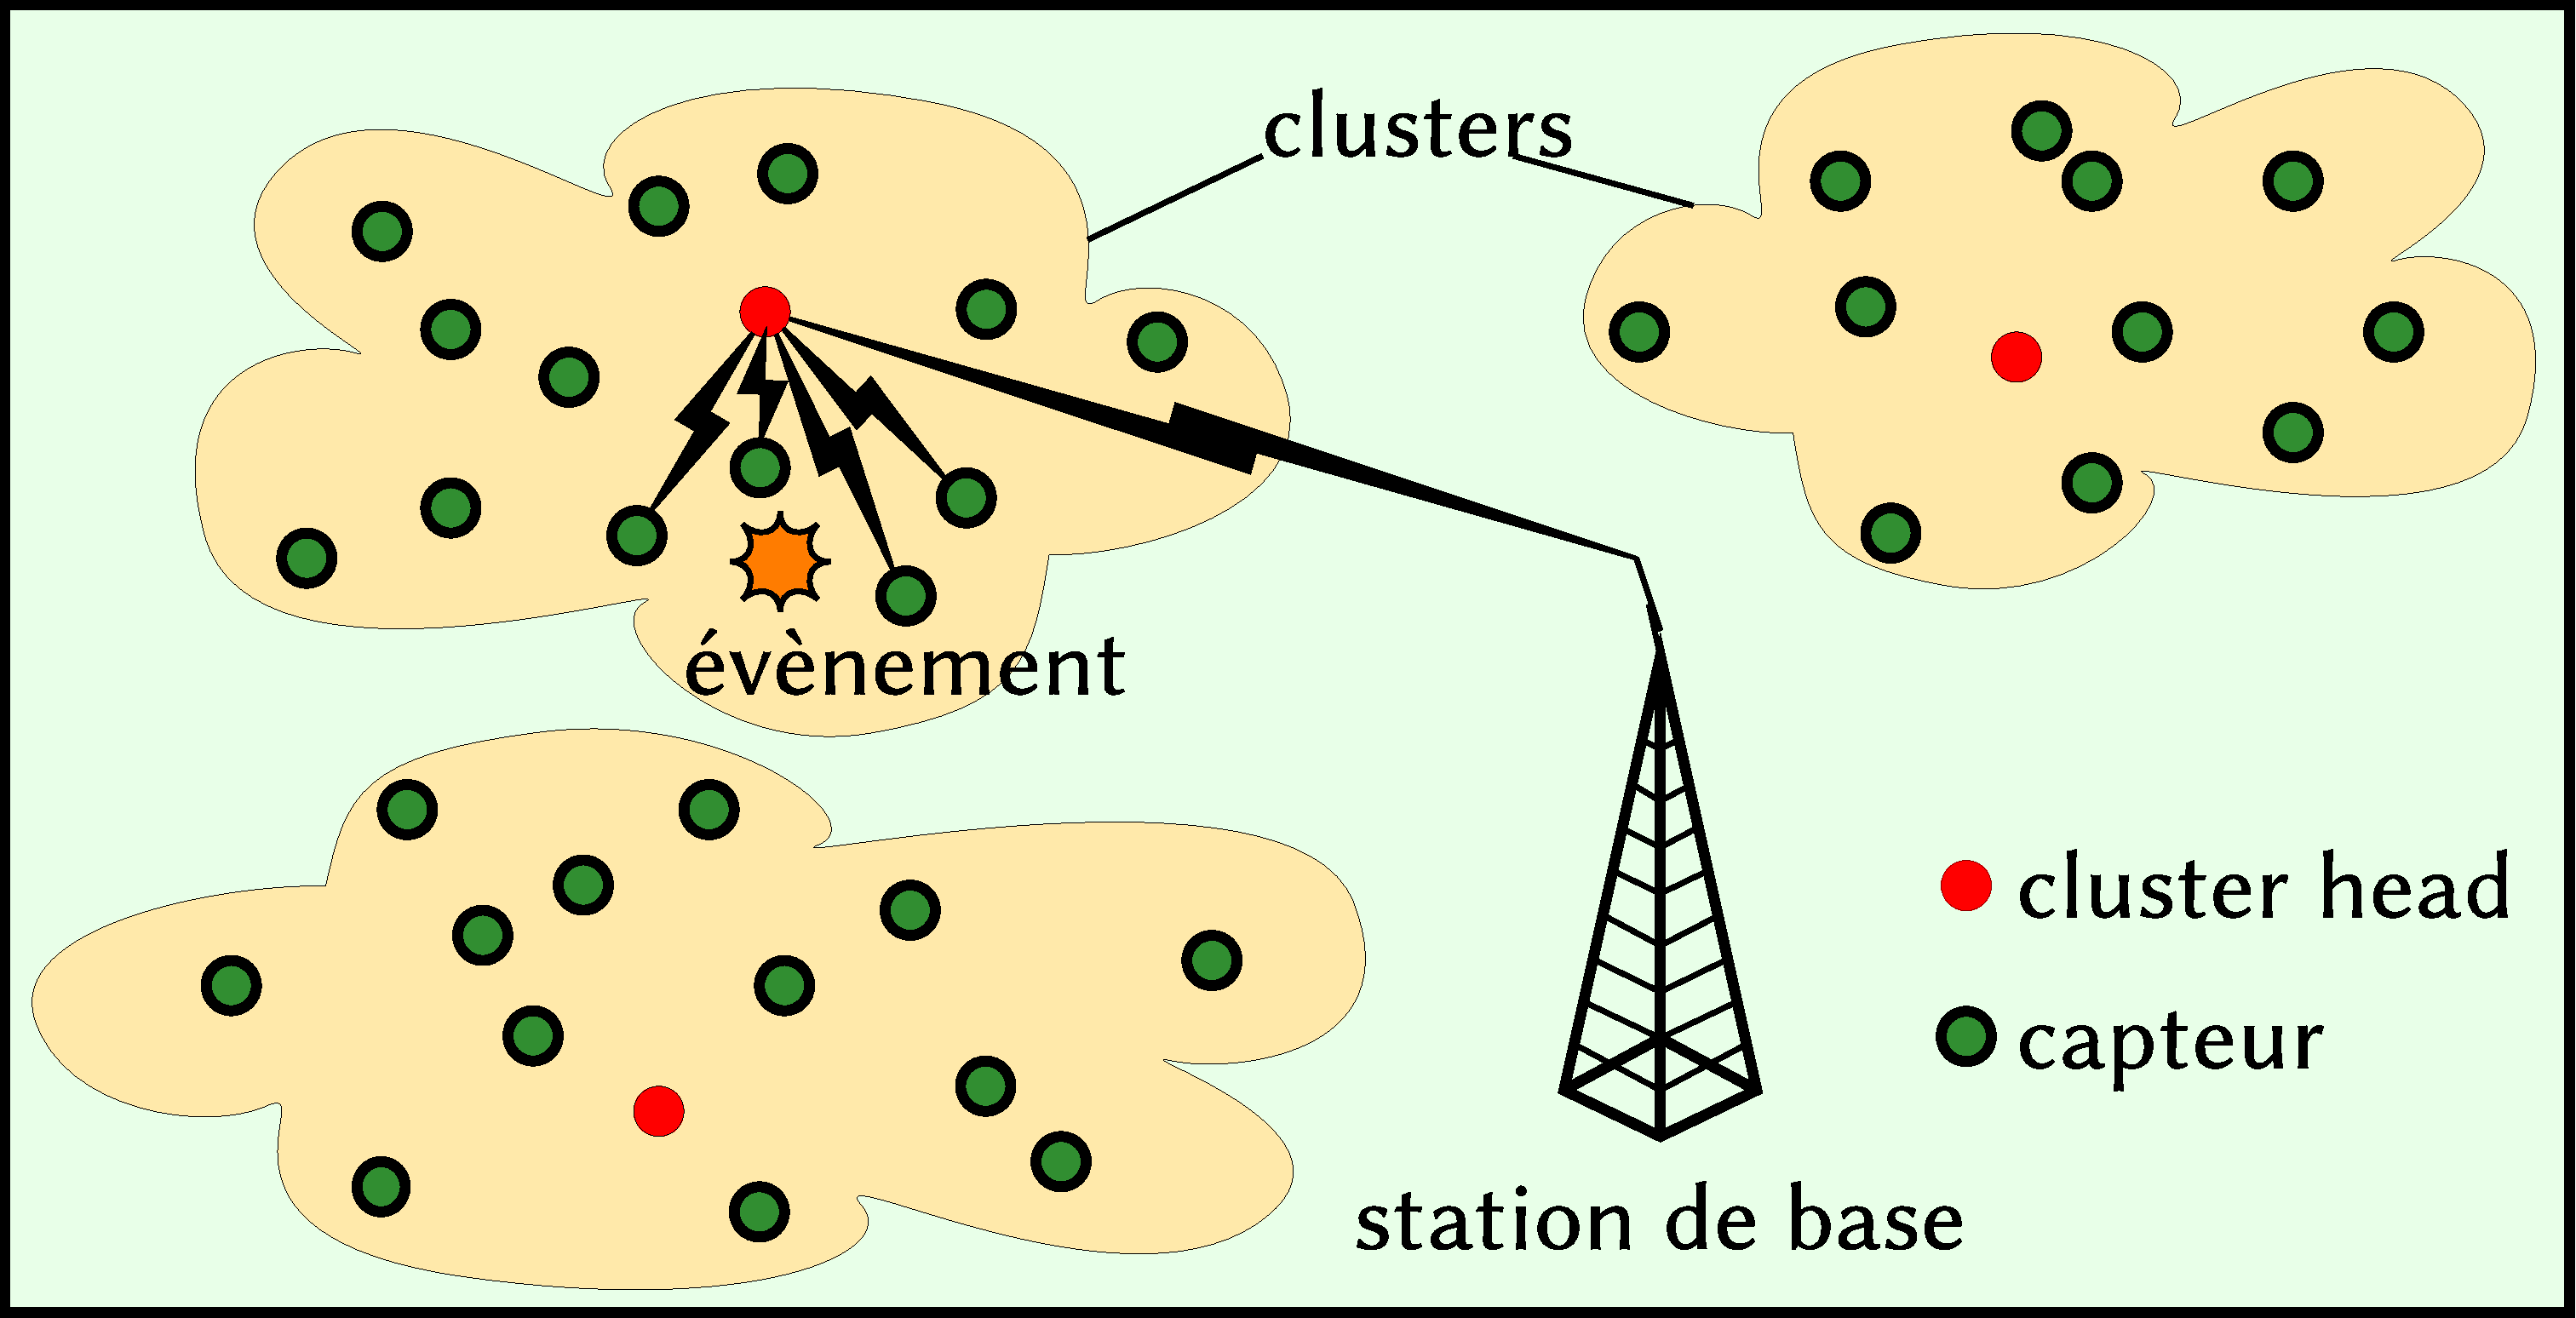
\includegraphics[width=0.8\linewidth]{\chapterfig/WSN.pdf}
    \caption{Schéma d'un \rc clusterisé}\label{st:fig:wsn}
\end{figure}

L'appel à un algorithme de «\idx{clusterisation}» a pour effet de limiter les émissions à «longue portée» (relativement aux communications intra-clusters) aux \chs seulement.
Or les communications sur de plus grandes distances se traduisent par une plus grande consommation en énergie (puisqu'une plus grande puissance d'émission est nécessaire).
Les capteurs normaux (non \chs) n'ont pas à atteindre directement des nœuds situés en dehors de leur cluster; ils économisent d'autant en énergie.
De plus, les \chs sont idéalement placés pour réaliser des opérations d'\idx{agrégation} voire de \idx{compression} sur les paquets qu'ils reçoivent, afin de limiter encore le volume des retransmissions couteuses en énergie.

À part les économies substantielles en énergie, la clusterisation d'un réseau présente plusieurs autres avantages:
\begin{itemize}
    \item elle permet de déployer une gestion «centralisée» d'un cluster, puisque le \ch est à même d'appliquer un algorithme tenant compte de tous les capteurs de son groupe. Pour autant, la topologie décentralisée de l'ensemble du réseau n'est pas sacrifiée, car les clusters sont indépendants de la \sdb, qui n'intervient pas dans leur fonctionnement interne;
    \item elle permet de gagner en \idx{extensibilité}, puisqu'il est aisé de rajouter des clusters au réseau, voire peu contraignant de rajouter des nœuds dans un cluster donné. L'évolution du réseau est ainsi plus simple à assurer que s'il fallait modifier un algorithme distribué pour prendre en compte l'intégration de nouveaux capteurs.
\end{itemize}
%2}}}

        \subsubsection{Clusterisation hiérarchique\index{clusterisation!clusterisation hiérarchique}}
%{{{2
Une fois le \rc divisé en clusters, rien n'empêche de considérer les clusters un à un et de leur appliquer à nouveau un algorithme de \idx{clusterisation}, de façon à établir des sous-ensembles dans chaque cluster.
Et ainsi de suite, de façon récursive, jusqu'à atteindre le degré de hiérarchie désiré.
L'intérêt de cette méthode est de créer une partition hiérarchique dans le réseau, permettant un meilleur contrôle des sous-ensembles de capteurs.
Par ailleurs, les clusters situés tout en bas dans la hiérarchie constituée seront de petite taille.
Les communications intra-clusters seront donc peu consommatrices en énergie.

Pour pouvoir distinguer plus facilement le niveau de hiérarchie auquel nous nous plaçons, nous désignerons par la suite sous le terme \textit{$k$-cluster} ($0 \leq k \leq$~nombre de capteurs) un sous-ensemble obtenu après $k$ applications de l'algorithme de \idx{clusterisation}.
En suivant cette convention, l'unique $0$-cluster est alors le réseau tout entier.
Lorsque nous parlons simplement de \textit{clusters}, il faudra comprendre $1$-clusters; autrement dit, des clusters issus d'une partition simple, sans degré supplémentaire de hiérarchie.

De même, on désignera par $k$-\ch (ou bien par $k$-\CH) les \chs de chacun des $k$-clusters du réseau.
Le rôle de $0$-cluster pourra alors être attribué à la \sdb.
Chaque $k$-\CH reçoit des données (provenant soit de nœuds normaux si $k$ est le dernier degré de la hiérarchie constituée, soit de ($k+1$)-\CH), les agrège et les transmet au ($k-1$)-\CH auquel il est rattaché.
%2}}}

        \subsubsection{Un exemple: fonctionnement de l'algorithme \leach}\label{st:subsubsec:leach}
%{{{2
L'un des algorithmes de \idx{clusterisation} les plus simples et les plus couramment employés dans les \rcsfs est l'algorithme \leach (\textit{Low Energy Adaptive Clustering Hierarchy}, \cad «hiérarchie de clusterisation adaptative à faible énergie» en anglais)~\cite{HCB00}.
Il s'agit d'un algorithme dynamique (il effectue de nouvelles clusterisations\index{clusterisation} du réseau régulièrement dans le temps) qui, par la formation de clusters, met en place une solution de routage simple mais efficace des paquets dans le réseau.

Voici le fonctionnement détaillé de cet algorithme.
Soit $P$ le pourcentage moyen de clusters désirés pour le réseau à un instant quelconque $t$.
\leach est découpé (dans la durée) en cycles, chacun constitué de $\frac{1}{P}$~rondes.
Chaque ronde $r$ est organisée de la façon suivante:
\begin{enumerate}
    \item Chaque nœud du réseau à partitionner calcule une valeur de seuil $S(i)$:
        \[
            S(i) = \left\{
            \begin{array}{cl}
                \displaystyle \frac{P}{1-P\cdot\left(r\mbox{ mod }\frac{1}{P}\right)} & \mbox{si }i\mbox{ n'a pas encore été \CH}\\
                                                                     0 & \mbox{si }i\mbox{ a déjà été \CH}
            \end{array}
            \right.
        \]
        Chaque nœud choisit un nombre pseudo-aléatoire $0 \le x_{i}\le 1$.
        Si $x_{i} \le S(i)$, alors $i$ s'auto-désigne comme \CH pour la ronde en cours.
        Il est à noter que le calcul de $S(i)$ est réalisé de telle façon que chaque nœud devienne \ch une fois et une fois seulement au cours de chaque cycle de $\frac{1}{P}$~rondes: le taux de probabilité d'auto-désignation $S(i)$ est égal à $1$ lorsque la fin du cycle est atteinte (autrement dit, lorsque $r = \frac{1}{P}-1$).
    \item Les \chs auto-désignés informent leurs nœuds voisins de leur changement de statut à l'aide de messages en diffusion générale (\textit{broadcast}).
        Tous ces messages sont envoyés en utilisant la même puissance de transmission (valeur fixe et prédéterminée lors de l'implémentation).
        Pour limiter les collisions, il est fait usage de la méthode \textit{Carrier Sense Multiple Access} (\csma) au niveau de la couche MAC.
    \item Les autres nœuds, qui ne se sont pas désignés en tant que \chs pour la ronde en cours, choisissent de se joindre au cluster du \CH dont ils perçoivent le signal avec l'intensité la plus élevée, \cad le \CH le plus proche en termes de puissance du signal électromagnétique.
        Chaque nœud prévient le \ch qu'il décide de rejoindre en lui envoyant un message.
        La méthode \csma est là encore appliquée.
    \item Au vu des réponses reçues, chaque \ch calcule un «ordre de transmission» pour les nœuds qui l'ont rejoint.
        Il annonce alors à chacun de ces nœuds l'instant auquel le nœud doit lui transmettre ses données.
        Dans chaque cluster, les nœuds s'adresseront donc à leur \ch à tour de rôle, selon l'ordre déterminé par le \CH, ce qui revient à utiliser la méthode appelée \textit{Time Division Multiple Access} (\tdma).
    \item La phase de collecte des données peut débuter.
        Les \chs restent en écoute et reçoivent les données des autres capteurs de leur cluster.
        Les capteurs «normaux» effectuent leur mission (ils réalisent des mesures sur leur environnement), et envoient leurs résultats au \ch lorsque c'est à leur tour de le faire.
        Quand ce n'est pas à leur tour de communiquer, ces nœuds mettent leur équipement radio en veille afin d'économiser leur énergie.
        Les collisions entre les transmissions des nœuds de différents clusters sont évitées grâce à la méthode appelée \textit{Code Division Multiple Access} (\cdma).
    \item Au fur et à mesure qu'ils reçoivent les données, les \chs agrègent\idx{agrégation}, et éventuellement compressent\idx{compression} ces dernières.
        Ils les envoient ensuite à la \sdb, soit au cours d'une unique transmission directe, soit en faisant relayer les paquets par d'autres \chs.
    \item Les étapes~5 et~6 sont répétées jusqu'à la fin de la ronde.
\end{enumerate}

Quelques remarques sont à énoncer.
Tout d'abord: pour un cluster donné, il est alors possible de réitérer l'application de l'algorithme \leach, afin de créer une nouvelle partition au sein même d'un cluster.
Et ainsi de suite par récursivité, jusqu'à obtenir le degré de hiérarchie\index{clusterisation!clusterisation hiérarchique} désiré dans le réseau.
Nous appellerons $k$-\leach cet algorithme appliqué de façon à créer $k$ degrés hiérarchiques.

Second point: l'un des aspects importants de \leach est que lors de la première étape, chaque nœud choisi d'être, ou non, un \ch pour la ronde en cours.
Ce choix est basé uniquement sur la valeur de seuil calculée, et sur le nombre pseudo-aléatoire généré; à aucun moment un nœud ne fait intervenir dans sa décision le comportement de ses voisins.
En conséquence, le pourcentage $P$ de \chs désirés dans le réseau n'est qu'une valeur moyenne sur l'ensemble des rondes de chaque cycle.
Par ailleurs, la répartition géographique (au regard de la puissance de transmission nécessaire) idéale des \chs n'est en rien assurée.
Au contraire, il est même probable d'obtenir, pour certaines rondes, une concentration importante de \chs dans une zone restreinte du réseau, tandis que d'autres régions seront mal couvertes.
Il n'y a pas grand-chose à faire dans ce cas, sinon espérer que la prochaine ronde produira une distribution des \CHs plus favorable.
Si toutefois un nœud ne parvient à capter les messages d'aucun \CH, il se déclare généralement lui-même \ch.
%2}}}

        \subsubsection{De nombreux algorithmes de \idx{clusterisation}}
%{{{2
De nombreux algorithmes de \idx{clusterisation} de données existent.
Plusieurs d'entre eux sont même spécifiquement adaptés aux \rcsfs.
C'est le cas de \leach qui prend place, comme évoqué plus haut, parmi les plus fréquemment utilisés, à tel point qu'il en existe de nombreuses variantes.
Par exemple, il est possible d'étendre l'algorithme pour prendre en compte l'énergie restante dont dispose chaque nœud lors de l'élection des \CH.
Cette énergie résiduelle intervient alors en temps que paramètre supplémentaire lors du calcul de la valeur de seuil $S(i)$~\cite{HHT02}.
D'autres travaux sont basés sur \leach, que ce soit pour améliorer ses performances~\cite{RR13,CJ14} ou bien sa sécurité~\cite{OFVWBDL07}.

Mais on trouve également de nombreux autres protocoles~\cite{AY07,DQWH13}.
Certains d'entre eux prennent en compte deux à trois paramètres, comme l'énergie résiduelle des nœuds, leur distance aux \chs potentiels et/ou le nombre de voisins de ces derniers: c'est le cas du protocole \heed~\cite{YF04}, assez souvent utilisé, ou du protocole MPC~\cite{KTAA12}, plus récent et moins répandu, se basant sur les k-moyennes.
Un quatrième élément, la confiance portée au nœud, est même utilisé parfois pour réaliser une sélection plus sure des \CH~\cite{KMSL09}.

Certains protocoles ont des buts plus précis, comme \ffuca~\cite{FL11,FMMMI12} qui repose sur l'exploitation de propriétés ultramétriques dans le réseau afin de créer une répartition «idéale» des nœuds dans les clusters en fonction de leur distance aux \CH; ou bien comme VSR~\cite{TV08}, créé à l'intention des \idx{MANET}, qui à l'aide d'une structure virtuelle détermine un routage proactif pour l'intérieur des clusters (ou les nœuds émettent au \ch en plusieurs sauts) et à la demande sur l'épine dorsale du réseau qui relie entre eux les \CH\,\footnote{Pour conserver la lisibilité du paragraphe, le développement des acronymes HEED, FFUCA, MPC et VSR n'est pas donné ici. Il est néanmoins disponible \hyperref[acronymes]{en fin d'ouvrage}.}.
\nomenclature{LEACH}{\textit{Low-Energy Adaptive Clustering Hierarchy}}
\nomenclature{HEED}{\textit{Hybrid, Energy-Efficient Distributed clustering}}
\nomenclature{FFUCA}{\textit{Fast and Flexible Unsupervised Clustering Algorithm }}
\nomenclature{MPC}{\textit{Multiple Parameter based Clustering}}
\nomenclature{VSR}{\textit{Virtual Struture Routing protocol}}
%2}}}
%1}}}

    \subsection{Déploiement autonome, \idx{mobilité}}
%{{{1
%{{{2
Les capteurs doivent être à même d'établir seuls une organisation autonome du réseau: ils comptent sur les protocoles inscrits dans leur mémoire, mais non sur une intervention externe (de l'administrateur par exemple).
L'organisation présente un défi en soi~\cite{TV08}, auquel les nombreux protocoles de découvertes des voisins et les algorithmes de \idx{routage} proposés au fil des ans apportent autant de réponses~\cite{DQWH13}.
Par ailleurs, ces protocoles sont tenus de gérer le départ ou l'arrivée de nouveaux nœuds dans le réseau.
C'est ce que l'on appelle l'\idx{extensibilité} du réseau (ou bien son évolutivité, ou encore sa scalabilité; \textit{scalability} est le terme anglais dénotant ce concept).

Qui plus est, il n'y a pas que le routage, mais l'intégralité de la chaine des opérations à réaliser qui doit être mise en place de façon autonome: la collecte de données en fait ainsi partie~\cite{ZWPT10}.
Un autre paramètre à gérer parfois est la \idx{mobilité} des nœuds.
Cette mobilité est une capacité propre aux \manet (\textit{Mobile Ad hoc Networks}, «réseaux ad hoc mobiles»).
Comme leur nom l'indique, il s'agit de \wanet dont les nœuds sont mobiles.
Lorsque ces nœuds sont (portés par) des véhicules, on parle même de \vanet (\textit{Vehicular Ad hoc Networks}, «réseaux ad hoc véhiculaires»).
Ces réseaux ont leurs propres problématiques~\cite{DYK12}, qui sont souvent assez proches de celles des \rcsfs.
Certaines solutions développées pour les \manet, des mécanismes de sécurité par exemple, peuvent tout à fait être réutilisés dans les \rcs~\cite{BMS13}.

Mais revenons à la \idx{mobilité} en elle-même: elle n'est pas systématique dans les \rcsfs, sont les nœuds sont la plupart du temps statiques ou quasiment statiques.
Il arrive néanmoins que des réseaux soit constitués, en intégralité ou bien en partie, par des capteurs mobiles.
Le fait de se retrouver dans un environnement où les distances et les vitesses évoluent continuellement rend accessibles de nouvelles applications, mais vient bien sûr compliquer le \idx{routage}, la collecte des données, et même la gestion de la \idx{mobilité} des nœuds (s'ils n'ont pas de pilotes humains par exemple, il faut éviter les collisions~\cite{E-ZCGGK12}).
Dans le cas de \rcs comportant des nœuds mobiles, le modèle du réseau se verra en général rattaché aux \manet et, bien que ne bénéficiant pas forcément des mêmes ressources, ce sont les mêmes algorithmes de \idx{routage} qui vont être utilisés pour assurer l'acheminement des paquets de bout en bout.
Nous reviendrons plus loin sur des solutions reposant sur un nombre restreint de nœuds mobiles se déplaçant au sein d'un réseau de capteurs fixes pour réaliser différentes opérations sur les appareils (collecte de données, diffusion d'information, réinitialisation de la configuration d'origine, \etc)~\cite{HR13}.
\nomenclature{MANET}{\textit{Mobile Ad hoc NETworks}}
\nomenclature{VANET}{\textit{Vehicular Ad hoc NETworks}}
%2}}}
%1}}}

    \subsection{Sécurité, \idx{sureté} et \resilience}
%{{{1
        \subsubsection{Sureté, \resilience}
%{{{2
Comme évoqué précédemment, une fois déployés, les \rcs doivent s'organiser et fonctionner seuls, sans intervention humaine.
Pour autant, ils ne sont pas à l'abri des erreurs ni des pannes.
L'idéal est donc de pouvoir assurer un certain degré de \idx{sureté} et de \resilience au réseau.

La \idx{sureté} d'un système est sa capacité à fonctionner sans erreurs, c'est à dire sans dysfonctionnement dus à une mauvaise conception ou à une mauvaise implémentation des architectures matérielle et logicielle.
Elle est en principe apportée soit par des tests en amont du déploiement, soit par une modélisation formelle (ou semi-formelle) du système, qui permet d'en évaluer certaines propriétés et de déduire, en fin de compte, si le système mis en place respecte ou non les spécifications établies.

Les tests et simulations sont récurrentes dans la quasi-totalité des travaux de la littérature.
Ils consistent à implémenter le dispositif étudié, physiquement ou virtuellement, pour étudier son évolution au cours d'une exécution «classique» ou bien soumise à des conditions d'expérimentation particulières.
Certains travaux ont même pour objet des tests comparatifs sur différentes architectures matérielles de capteurs~\cite{PLP06}, ou encore recensent les différents systèmes de simulation permettant d'expérimenter sur les réseaux de capteurs~\cite{AAAHN12}.

Pour la vérification basée sur des méthodes formelles, des outils tels que le \idx{\textit{model checking}} peuvent par exemple être appliqués sur le modèle établi.
Le \textit{model checking} est une technique pouvant être utilisée sur des systèmes concurrents à états finis, et qui permet d'extraire automatiquement certaines propriétés sur les performances ou la sureté du modèle puis de s'assurer qu'elles sont respectées dans le réseau à tout instant.
Si le système ne fonctionne pas comme prévu, l'outil permet parfois d'obtenir une trace qui vient faciliter la localisation de la source de l'erreur.
Contrairement aux tests et aux simulations, les résultats obtenus à l'aide du \idx{\textit{model checking}} ne varient pas entre deux instances.
Encore mieux: la spécification formelle du système permet de vérifier les propriétés sur tous les cas possibles d'exécution déterminés par les spécifications du modèle, tandis que des simulations ne permettent de remonter que certaines erreurs détectées (sans assurance de les avoir trouvées toutes).
Le \textit{\idx{model checking}} est utilisé régulièrement dans les réseaux sans fils, que ce soit pour valider la conception de protocoles de routage comme pour la vérification de propriétés de sureté concernant les risques de collisions au sein d'un groupe de véhicules~\cite{E-ZCGGK12}.
%2}}}

        \subsubsection{Résilience}
%{{{2
La \resilience d'un système est la capacité de ce système à outrepasser et éventuellement à corriger les erreurs susceptibles de survenir.
Autrement dit, un système résilient est capable de poursuivre son fonctionnement avec toujours autant d'efficacité ou presque, même si des pannes matérielles, des erreurs logicielles ou d'autres types d'incidents viennent perturber le système.
Assurer la \resilience revient donc à anticiper, à prévoir des «plans de secours», des mécanismes de correction et de réparation automatiques.

Concrètement, dans un \rcsfs, elle met en jeu des principes comme la redondance des données stockées et envoyées, des routes de retransmission~\cite{SP10}; elle s'établit sur l'usage de protocoles capables de se mettre à jour lorsque des nœuds disparaissent (épuisement supposé) ou apparaissent (nouveaux arrivants) dans le réseau, de mécanismes de correction d'erreurs…
La résilience matérielle passe le plus souvent par la redondance des composants, mais n'est que rarement mise en place, pour des raisons de couts, dans les \rcs.
On préféra en général utiliser quelques capteurs en plus par rapport à la quantité strictement nécessaire pour assurer le service, sans avoir à augmenter le prix de \emph{tous} les capteurs.

La sureté et la résilience des réseaux ne sont pas des problématiques de sécurité (car aucune attaque volontaire ne rentre en compte), mais il s'agit de problématiques assez proches de la disponibilité des réseaux (définie au \chapref{ea}, \ssref{ea:def:dispo}).
%2}}}

        \subsubsection{Sécurité}
%{{{2
En raison de leurs faibles capacités, conjuguées aux domaines critiques dans lesquels ils interviennent parfois, les capteurs peuvent présenter des cibles de choix pour un attaquant.
Les algorithmes et mécanismes classiques utilisés en \idx{cryptographie} afin d'assurer la confidentialité ou l'authentification des données sont souvent très exigeants en ressources (en termes de calculs notamment, et donc de consommation énergétique).
Il a fallu adapter ces mécanismes aux capteurs.

D'autres attaques peuvent être menées, non plus pour intercepter des données, mais dans le but de perturber le bon fonctionnement du réseau.
Ce sont les attaques dites de \textit{\dds}.
Un attaquant, par le biais d'un nœud compromis par exemple, peut ainsi chercher à détourner des flux de données au sein du réseau, à empêcher des paquets de parvenir à destination (en les supprimant), à maximiser le débit du nœud compromis au détriment de celui des autres nœuds, à saturer le canal de transmission pour empêcher les nœuds légitimes de l'utiliser, ou encore à pousser les autres capteurs à l'épuisement de leurs réserves en énergie, \etc.
Pour rappel, l'objectif des travaux présentés dans cet ouvrage consiste à proposer, modéliser et tester une solution permettant de détecter, puis de réagir aux attaques de ce type, tout en assurant une consommation minimale en ressources pour les capteurs du réseau.

\paragraph{}
Bien que le thème de la \secu des \rcsfs, notamment sur le sujet des attaques de type «\dds» ainsi que des contre-mesures appropriées, ait tout à fait sa place dans ce chapitre, il s'agit d'un élément central pour les travaux de cet ouvrage, et il est développé avec beaucoup plus de précisions que les problématiques précédentes.
Aussi a-t-il été choisi de lui attribuer un chapitre spécifique: les pages qui suivent abordent la question de la \secu avec bien plus de détails que jusqu'à présent.
%2}}}
%1}}}

% vim: set spelllang=fr foldmethod=marker:
\section{Hypothèses de travail}

\todo{À déplacer en \chapref{in} ou en début de \chapref{sa}? Terminologie entre sections 1 et 2 de ce chapitre?}

    \subsection{Terminologie employée}

        \paragraph{Capteurs et nœuds}
Un \rcsf est souvent représenté sous forme de graphe.
En conséquence, il est souvent fait références aux capteurs eux-mêmes sous le terme de « nœuds ».
Nous parlerons plutôt de capteurs lorsque nous évoquerons les « \rcs » eux-mêmes, ainsi que les mesures physiques qu'ils réalisent sur leur environnement, et plutôt de nœuds lorsque nous sommes amenés à travailler sur des graphes.
Mais la plupart du temps, ces deux termes peuvent être employés dans cette thèse de manière complètement interchangeable.
Leur alternance n'a le plus souvent que pour but de limiter les répétitions au sein d'une phrase.

        \paragraph{Nœuds normaux}
Les « nœuds normaux » ont deux significations possibles selon le contexte.
\begin{enumerate}
    \item Lorsqu'il est question de partition, de « clusterisation » du réseau, un nœud \textit{normal} est un nœud qui n'a pas été sélectionné pour assurer la fonction de « chef » du cluster, de \ch. De même lorsque des nœuds de contrôle (\cns ou \vns) ont été sélectionné, les nœuds \textit{normaux} sont les nœuds qui n'ont pas été sélectionnés (ni comme nœud de contrôle, ni comme \ch): ils poursuivent donc simplement leur rôle de collecte et de transmission des données mesurées.
    \item Lorsqu'il est question de \secu et d'attaques menées depuis l'intérieur du réseau, un nœud \textit{normal} désigne un nœud non compromis. Les termes « nœud légitime », « nœud sain » ont le même sens dans cette thèse. Ils sont à opposer au nœud « attaquant », « compromis », « corrompu » ou occasionnellement « cupide ».
\end{enumerate}

        \paragraph{Attaquant}
Le terme d'« attaquant » fera le plus souvent référence à l'entité consciente qui se trouve à l'origine d'une attaque, qu'il s'agisse d'une personne seule ou d'une organisation.
Il arrive toutefois que par abus de langage, l'\textit{attaquant} soit utilisé comme un raccourci pour « le nœud attaquant », c'est à dire le nœud corrompu par l'\textit{attaquant} réel, depuis lequel l'attaque est menée au sein du réseau.

        \paragraph{Exploitant}
L'\textit{exploitant} du réseau désignera l'entité (entité humaine ou organisation) qui exploite le \rcsfs: l'entité qui interagit avec la \sdb, de l'« autre côté » du réseau, pour récupérer et analyser les données collectées par les capteurs et remontées jusqu'à la \BS.
Sauf précision contraire, on fera généralement l'amalgame avec l'\textit{administrateur} du réseau, qui procède directement à sa mise en place et éventuellement à son maintien en fonction.

        \paragraph{Des capteurs conscients!}
Il va de soi qu'un capteur est un appareil dépourvu de vie et de conscience.
Par abus de langage, des raccourcis sont parfois empruntés dans cette thèse et leur prêtent des intentions ainsi qu'une durée de vie.
Ainsi il arrive que les capteurs « cherchent à », « essayent de », « veulent » réaliser des actions; ou bien qu'ils « prétendent » être de meilleurs candidats au poste de \ch.
De même, ils sont susceptibles de « mourir » lorsque leur batterie est épuisée.
Ces tournures, bien qu'abusives en termes d'exactitude du langage, permettent en général de simplifier les explications.


\bigskip
\todo{Mobilité, hypothèses (protocoles), etc.}


Beside being energy-efficient, it is important for an algorithm to \emph{just work}, and thus for researchers to provide guaranties of its functioning.
Formal method may help in this, and one of the most interesting techniques is model-checking.
It is a formal method based technique for verifying finite-state-concurrent systems, and can automatically extract performance or safety properties from a model and to ensure they are asserted at all time in the network.
Additionally, were a system not to work properly, model-checking tools provide a trace to help finding the source of the error.
Contrary to testing or simulation, results obtained \via model-checking do not vary between distinct running instances; more important, formal specification enables one to verify the system against every single execution trace, where testing would only raise some encountered errors (maybe not all existing errors).
Model-checking is used in a wide area of applications, from the validation of network protocols to the verification of safety properties in regard with the non-collision between platoon vehicles\cite{E-ZCGGK12}, for example.

One of the two aforementioned papers already makes use of formal methods, including model-checking, to evaluate its proposal\cite{BMM13}.
A first attempt is described in the study to model it with CTMC (Continuous Time Markov Chains), but limitations due to the period over which the detection is performed led to put away Markovian processes.
Instead the nodes and the monitoring agents are modeled with eGSPN (extended Generalized Stochastic Petri Networks), a class of Petri networks including times transitions and suitable for representing stochastic processes.
From those eGSPNs we could extract a number of performance and dependability properties formally expressed in terms of the Hybrid Automata Stochastic Logic (HASL\cite{BDDHP11hasl}) and relying on Linear Hybrid Automata (LHA).
These properties were eventually asserted with the COSMOS statistical model-checker\cite{BDDHP11cosmos}.

Other works include model-checking of WSN-addressed systems, though we found few of them concerning protection against \DoS attacks.
In~\cite{TCCDC09} for example, three security protocols are analyzed through model-checking, nominally TinySec, allowing authentication and encryption, and LEAP and TinyPK, both used for key management. 
The authors used the AVISTA model-checker, designed for verifying security protocols.
In our study, we prefer to work with the more general UPPAAL model-checking tool.


\bigskip


A lot of approaches intended to bring security in a WSN are cluster-based~\cite{GD14}.
But the main purpose of clustering a sensor network usually resides in scaling possibilities, improved nodes management and energy savings brought by partitioning.
Several clustering algorithms have been proposed~\cite{AY07}.
They generally aim at determining which nodes in the network will be the \chs, often basing the choice on energetic considerations.
Basically, choosing a \ch in a network is not so different than selecting \cns in a cluster.
But in the latter case we have some additional constraints on security.

One of the easiest clustering algorithm to implement, and probably one of the most used is the \leach algorithm~\cite{HHT02}.
\leach makes each node draw a pseudo-random number and match it with a threshold which was computed from the number of desired \chs in the network and from the last iteration when the sensor was selected as a \CH.
There is a number of proposals derived from \leach, to improve either its efficiency~\cite{RR13,CJ14} or its security~\cite{OFVWBDL07}.
Other example clustering algorithms include HEED~\cite{YF04} or FFUCA~\cite{FMMMI12}.

Aside from clustering, the importance of energetic issues in WSNs have led to the proposals of several mechanisms to cut down its consumption~\cite{ACFP09}, based for example on packets priority~\cite{SAS14}.

\bigskip
\todo{Ambient backscatter (articles/A\_TRIER/)}\\

\todo{VSR\cite{TV08} dans protocoles clustering}
